\documentclass[11pt,a4paper]{report}
\usepackage[textwidth=37em,vmargin=30mm]{geometry}
\usepackage{calc,xunicode,amsmath,amssymb,paralist,enumitem,tabu,booktabs,datetime2,xeCJK,xeCJKfntef,listings}
\usepackage{tocloft,fancyhdr,tcolorbox,xcolor,graphicx,eso-pic,xltxtra,xelatexemoji}

\newcommand{\envyear}[0]{2025}
\newcommand{\envdatestr}[0]{2025-05-26}
\newcommand{\envfinaldir}[0]{webdb/2025/20250526/final}

\usepackage[hidelinks]{hyperref}
\hypersetup{
    colorlinks=false,
    pdfpagemode=FullScreen,
    pdftitle={Web Digest - \envdatestr}
}

\setlength{\cftbeforechapskip}{10pt}
\renewcommand{\cftchapfont}{\rmfamily\bfseries\large\raggedright}
\setlength{\cftbeforesecskip}{2pt}
\renewcommand{\cftsecfont}{\sffamily\small\raggedright}

\setdefaultleftmargin{2em}{2em}{1em}{1em}{1em}{1em}

\usepackage{xeCJK,xeCJKfntef}
\xeCJKsetup{PunctStyle=plain,RubberPunctSkip=false,CJKglue=\strut\hskip 0pt plus 0.1em minus 0.05em,CJKecglue=\strut\hskip 0.22em plus 0.2em}
\XeTeXlinebreaklocale "zh"
\XeTeXlinebreakskip = 0pt


\setmainfont{Brygada 1918}
\setromanfont{Brygada 1918}
\setsansfont{IBM Plex Sans}
\setmonofont{JetBrains Mono NL}
\setCJKmainfont{Noto Serif CJK SC}
\setCJKromanfont{Noto Serif CJK SC}
\setCJKsansfont{Noto Sans CJK SC}
\setCJKmonofont{Noto Sans CJK SC}

\setlength{\parindent}{0pt}
\setlength{\parskip}{8pt}
\linespread{1.15}

\lstset{
	basicstyle=\ttfamily\footnotesize,
	numbersep=5pt,
	backgroundcolor=\color{black!5},
	showspaces=false,
	showstringspaces=false,
	showtabs=false,
	tabsize=2,
	captionpos=b,
	breaklines=true,
	breakatwhitespace=true,
	breakautoindent=true,
	linewidth=\textwidth
}






\newcommand{\coverpic}[2]{
    % argv: itemurl, authorname
    Cover photo by #2~~(\href{#1}{#1})
}
\newcommand{\makeheader}[0]{
    \begin{titlepage}
        % \newgeometry{hmargin=15mm,tmargin=21mm,bmargin=12mm}
        \begin{center}
            
            \rmfamily\scshape
            \fontspec{BaskervilleF}
            \fontspec{Old Standard}
            \fontsize{59pt}{70pt}\selectfont
            WEB\hfill DIGEST
            
            \vfill
            % \vskip 30pt
            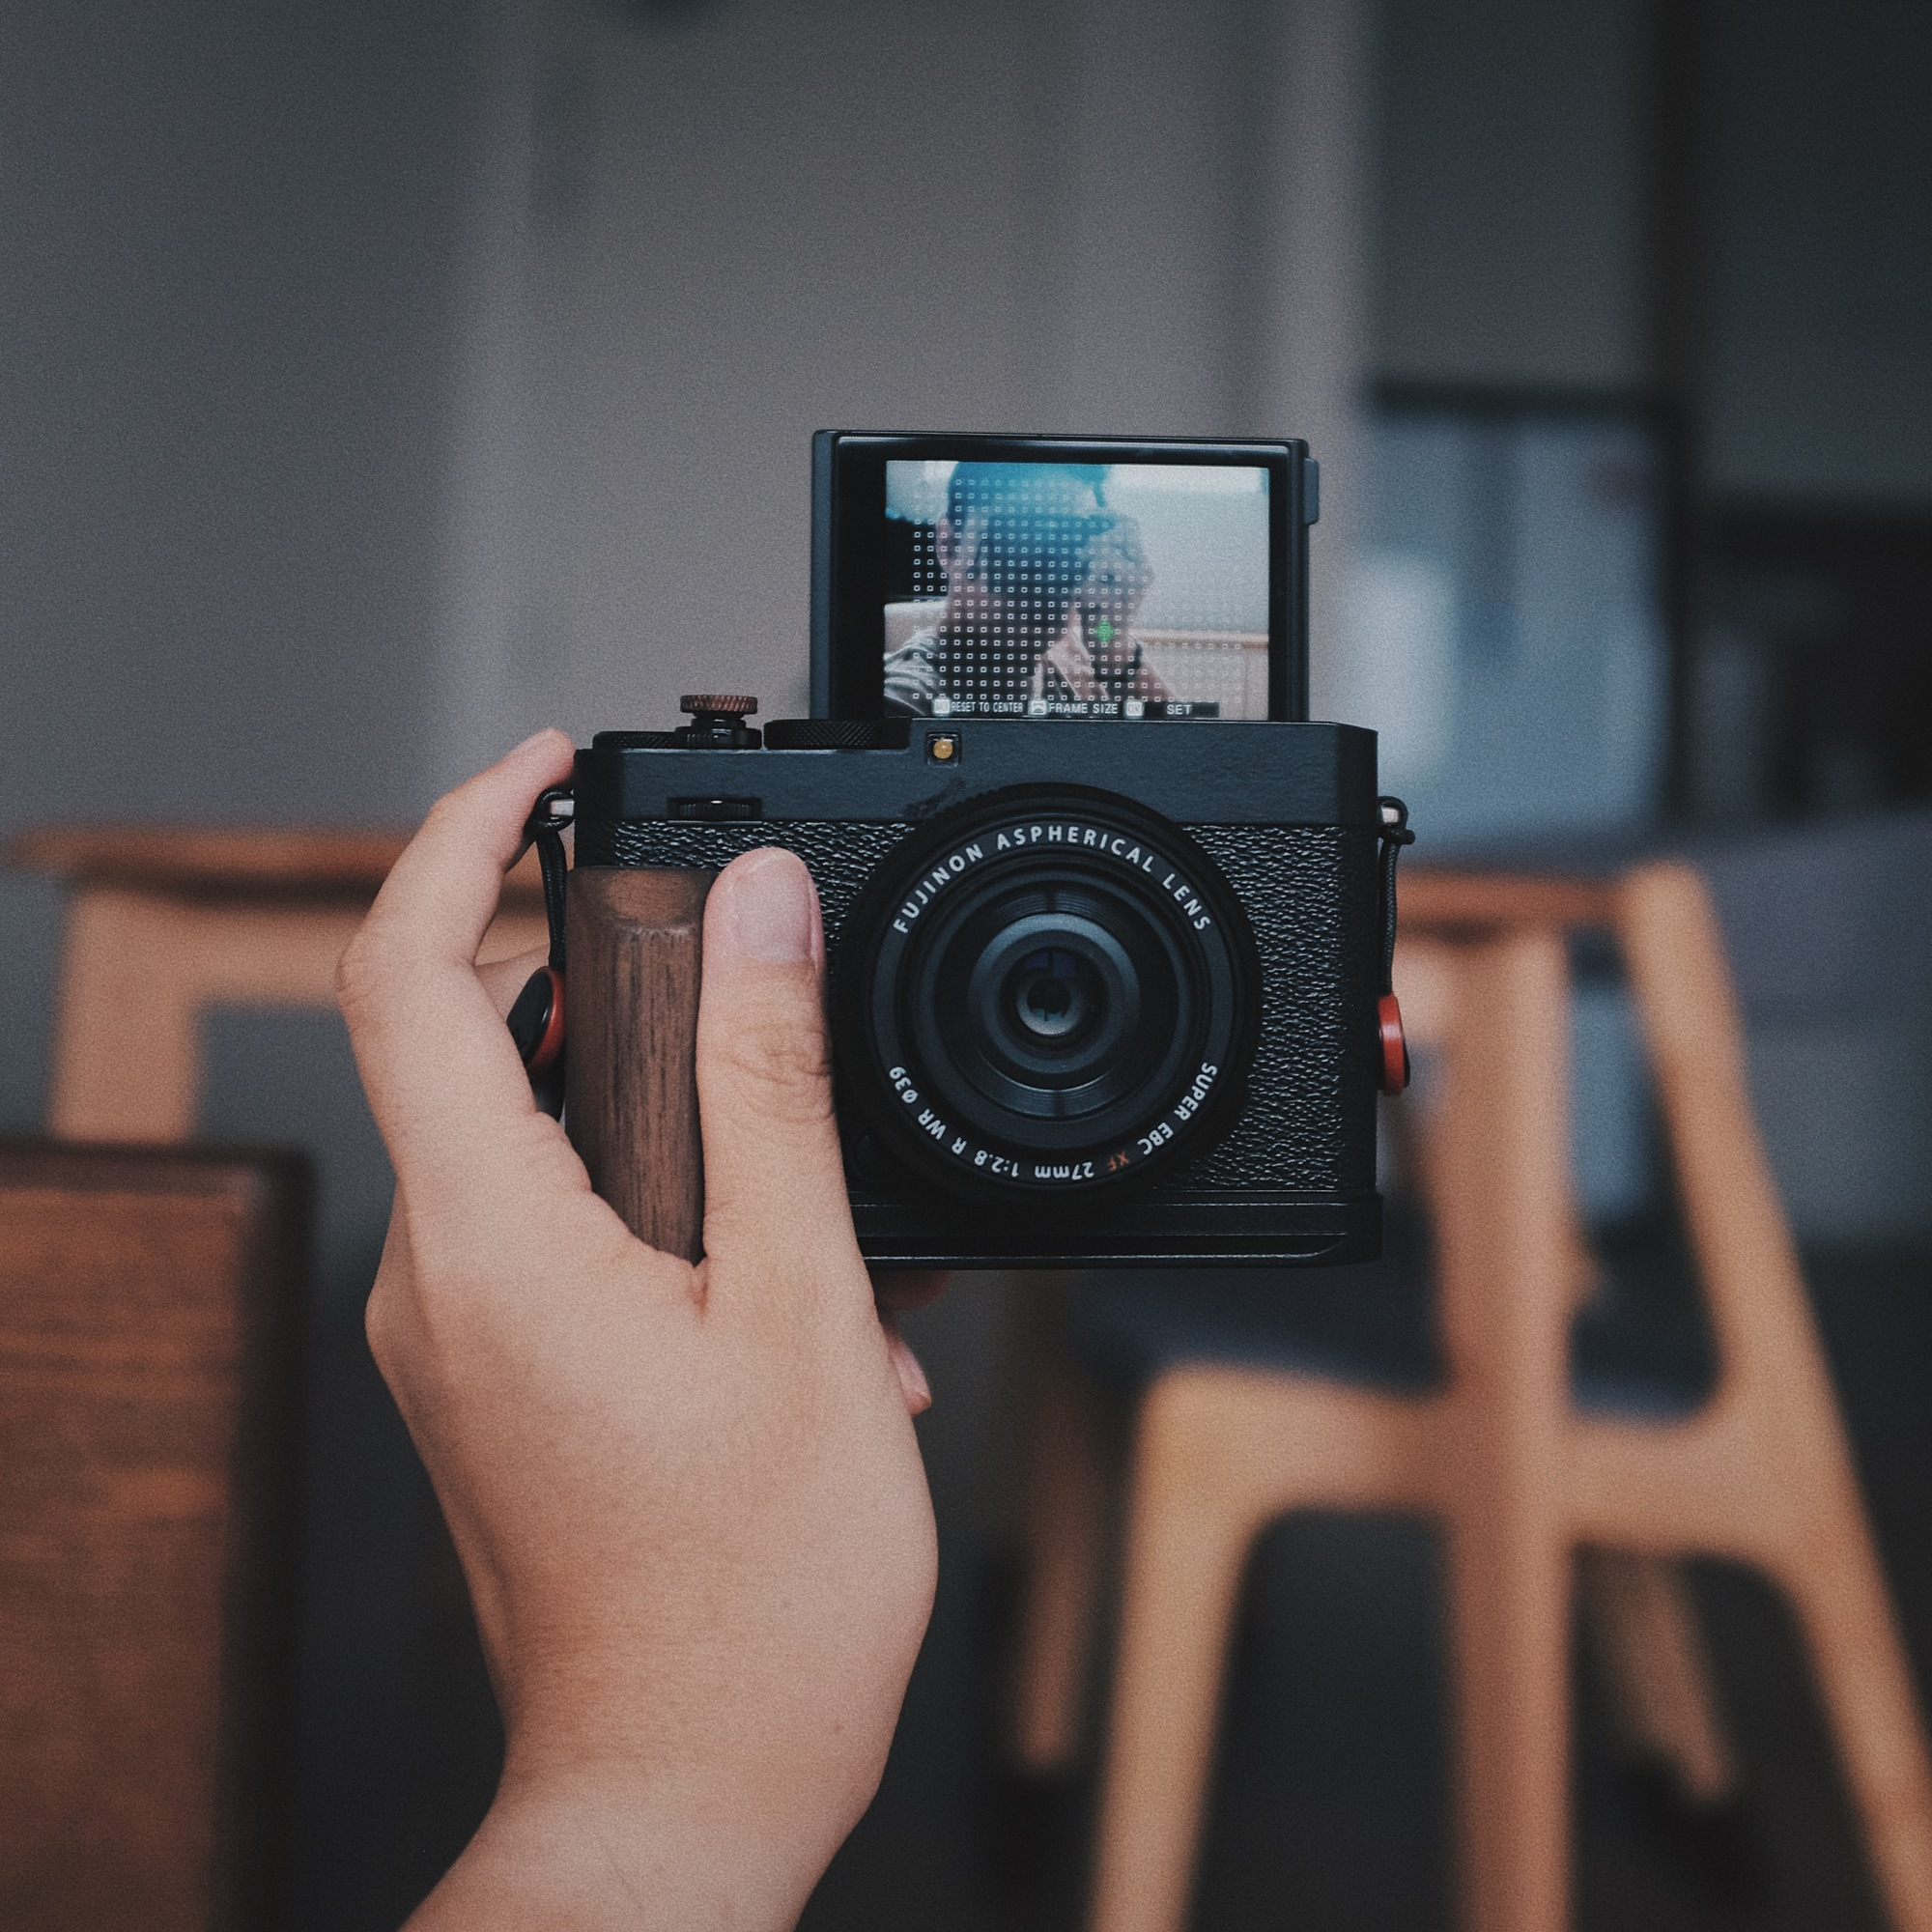
\includegraphics[width=\linewidth]{\envfinaldir/coverpic-prod.jpg}\par
            % \vskip 30pt
            \vfill

            \normalsize\rmfamily\scshape
            \copyright{} The Web Digest Project \hfill\large \envdatestr
        \end{center}
    \end{titlepage}
    % \restoregeometry
}
\newcommand{\simplehref}[1]{%
    \textcolor{blue!80!green}{\href{#1}{#1}}%
}
\renewcommand{\contentsname}{\center\Huge\sffamily\bfseries Contents\par\vskip 20pt}
\newcounter{ipartcounter}
\setcounter{ipartcounter}{0}
\newcommand{\ipart}[1]{
    % \vskip 20pt
    \clearpage
    \stepcounter{ipartcounter}
    \phantomsection
    \addcontentsline{toc}{chapter}{#1}
    % \begin{center}
    %     \Huge
    %     \sffamily\bfseries
    %     #1
    % \end{center}
    % \vskip 20pt plus 7pt
}
\newcounter{ichaptercounter}
\setcounter{ichaptercounter}{0}
\newcommand{\ichapter}[1]{
    % \vskip 20pt
    \clearpage
    \stepcounter{ichaptercounter}
    \phantomsection
    \addcontentsline{toc}{section}{\numberline{\arabic{ichaptercounter}}#1}
    \begin{center}
        \Huge
        \sffamily\bfseries
        #1
    \end{center}
    \vskip 20pt plus 7pt
}
\newcommand{\entrytitlefont}[1]{\subsection*{\raggedright\Large\sffamily\bfseries#1}}
\newcommand{\entryitemGeneric}[2]{
    % argv: title, url
    \parbox{\linewidth}{
        \entrytitlefont{#1}\par\vskip 5pt
        \footnotesize\ttfamily\mdseries
        \simplehref{#2}
    }\vskip 11pt plus 11pt minus 1pt
}
\newcommand{\entryitemGithub}[3]{
    % argv: title, url, desc
    \parbox{\linewidth}{
        \entrytitlefont{#1}\par\vskip 5pt
        \footnotesize\ttfamily\mdseries
        \simplehref{#2}\par\vskip 5pt
        \small\rmfamily\mdseries#3
    }\vskip 11pt plus 11pt minus 1pt
}
\newcommand{\entryitemAp}[3]{
    % argv: title, url, desc
    \parbox{\linewidth}{
        \entrytitlefont{#1}\par\vskip 5pt
        \footnotesize\ttfamily\mdseries
        \simplehref{#2}\par\vskip 5pt
        \small\rmfamily\mdseries#3
    }\vskip 11pt plus 11pt minus 1pt
}
\newcommand{\entryitemHackernews}[3]{
    % argv: title, hnurl, rawurl
    % \parbox{\linewidth}{
    %     \entrytitlefont{#1}\par\vskip 5pt
    %     \footnotesize\ttfamily\mdseries
    %     \simplehref{#3}\par
    %     \textcolor{black!50}{\href{#2}{#2}}
    % }\vskip 11pt plus 11pt minus 1pt
    \begin{minipage}{\linewidth}
            \entrytitlefont{#1}\par\vskip 5pt
            \footnotesize\ttfamily\mdseries
            \simplehref{#3}\par
            \textcolor{black!50}{\href{#2}{#2}}
    \end{minipage}\par\vskip 11pt plus 11pt minus 1pt
}







\begin{document}

\makeheader

\tableofcontents\clearpage




\ipart{Developers}
\ichapter{Hacker News}
\entryitemTwoLinks{Plwm – An X11 window manager written in Prolog}{https://news.ycombinator.com/item?id=44089424}{https://github.com/Seeker04/plwm}

\entryitemTwoLinks{Open Source Society University – Path to a free self-taught education in CS}{https://news.ycombinator.com/item?id=44089150}{https://github.com/ossu/computer-science}

\entryitemTwoLinks{The Newark airport crisis}{https://news.ycombinator.com/item?id=44089134}{https://www.theverge.com/planes/673462/newark-airport-delay-air-traffic-control-tracon-radar}

\entryitemTwoLinks{Denmark to raise retirement age to 70}{https://news.ycombinator.com/item?id=44088957}{https://www.telegraph.co.uk/world-news/2025/05/23/denmark-raise-retirement-age-70/}

\entryitemTwoLinks{Show HN: DaedalOS – Desktop Environment in the Browser}{https://news.ycombinator.com/item?id=44088777}{https://github.com/DustinBrett/daedalOS}

\entryitemTwoLinks{Writing your own CUPS printer driver in 100 lines of Python (2018)}{https://news.ycombinator.com/item?id=44088682}{https://behind.pretix.eu/2018/01/20/cups-driver/}

\entryitemTwoLinks{Lottie is an open format for animated vector graphics}{https://news.ycombinator.com/item?id=44088216}{https://lottie.github.io/}

\entryitemTwoLinks{Design Pressure: The Invisible Hand That Shapes Your Code}{https://news.ycombinator.com/item?id=44087844}{https://hynek.me/talks/design-pressure/}

\entryitemTwoLinks{At Amazon, some coders say their jobs have begun to resemble warehouse work}{https://news.ycombinator.com/item?id=44087150}{https://www.nytimes.com/2025/05/25/business/amazon-ai-coders.html}

\entryitemTwoLinks{Show HN: SVG Animation Software}{https://news.ycombinator.com/item?id=44087049}{https://expressive.app/expressive-animator/}

\entryitemTwoLinks{Claude 4 System Card}{https://news.ycombinator.com/item?id=44085920}{https://simonwillison.net/2025/May/25/claude-4-system-card/}

\entryitemTwoLinks{How to Install Windows NT 4 Server on Proxmox}{https://news.ycombinator.com/item?id=44084885}{https://blog.pipetogrep.org/2025/05/23/how-to-install-windows-nt-4-server-on-proxmox/}

\entryitemTwoLinks{CAPTCHAs are over (in ticketing)}{https://news.ycombinator.com/item?id=44084677}{https://behind.pretix.eu/2025/05/23/captchas-are-over/}

\entryitemTwoLinks{Failure Mechanisms in Democratic Regimes – An Army's Role}{https://news.ycombinator.com/item?id=44084653}{https://angrystaffofficer.com/2025/03/02/failure-mechanisms-in-democratic-regimes-an-armys-role/}

\entryitemTwoLinks{Scientific conferences are leaving the US amid border fears}{https://news.ycombinator.com/item?id=44084017}{https://www.nature.com/articles/d41586-025-01636-5}

\entryitemTwoLinks{Why old games never die, but new ones do}{https://news.ycombinator.com/item?id=44083917}{https://pleromanonx86.wordpress.com/2025/05/06/why-old-games-never-die-but-new-ones-do/}

\entryitemTwoLinks{Show HN: 1 min workouts for people who sit all day}{https://news.ycombinator.com/item?id=44083687}{https://shortreps.com}

\entryitemTwoLinks{Reinvent the Wheel}{https://news.ycombinator.com/item?id=44083467}{https://endler.dev/2025/reinvent-the-wheel/}

\entryitemTwoLinks{Tachy0n: The Last 0day Jailbreak}{https://news.ycombinator.com/item?id=44083388}{https://blog.siguza.net/tachy0n/}

\entryitemTwoLinks{Lone coder cracks 50-year puzzle to find Boggle's top-scoring board}{https://news.ycombinator.com/item?id=44082892}{https://www.ft.com/content/0ab64ced-1ed1-466d-acd3-78510d10c3a1}\ichapter{Phoronix}
\entryitemGeneric{\hskip 0pt{}Linux 6.15 Released With Continued Rust Integration, Bcachefs Stabilizing}{https://www.phoronix.com/news/Linux-6.15-Released}

\entryitemGeneric{\hskip 0pt{}ConfigFS Prepares Rust Support For Linux 6.16}{https://www.phoronix.com/news/Linux-6.16-ConfigFS}

\entryitemGeneric{\hskip 0pt{}Btrfs To See More Performance Improvements With Linux 6.16}{https://www.phoronix.com/news/Linux-6.16-Btrfs-Performance}

\entryitemGeneric{\hskip 0pt{}Dell Latitude 7455 Is The Newest Qualcomm Snapdragon X Elite Laptop Seeing Linux Patches}{https://www.phoronix.com/news/Dell-Latitude-7455-X1E-Linux}

\entryitemGeneric{\hskip 0pt{}Linux 6.16 Features Include A Lot From Intel, NVIDIA Blackwell, AMDGPU User Mode Queues}{https://www.phoronix.com/news/Linux-6.16-Features-Early-Look}

\entryitemGeneric{\hskip 0pt{}More Gaming Controllers From Turtle Beach \& PowerA Supported By Linux 6.15}{https://www.phoronix.com/news/Linux-6.15-Turtle-Beach-PowerA}

\entryitemGeneric{\hskip 0pt{}Rust Coreutils 0.1 Released With Big Performance Gains - Can Match Or Exceed GNU Speed}{https://www.phoronix.com/news/Rust-Coreutils-0.1-Released}

\entryitemGeneric{\hskip 0pt{}GNOME Web Making It Easier To Toggle WebKit Features}{https://www.phoronix.com/news/GNOME-Web-Toggle-Features}

\entryitemGeneric{\hskip 0pt{}Mike Blumenkrantz Axes Old Mesa Code: Goodbye Gallium Nine}{https://www.phoronix.com/news/Gallium-Nine-Removed-Mesa}


\ipart{Developers~~~~(zh-Hans)}
\ichapter{Solidot}
\entryitemGeneric{\hskip 0pt{}SteamOS 正式支持第三方掌机}{https://www.solidot.org/story?sid=81387}

\entryitemGeneric{\hskip 0pt{}亚马逊不再续订《时光之轮》第四季}{https://www.solidot.org/story?sid=81386}

\entryitemGeneric{\hskip 0pt{}马斯克的数据中心起火}{https://www.solidot.org/story?sid=81385}

\entryitemGeneric{\hskip 0pt{}为什么硅谷的科技右派痴迷于托尔金的作品}{https://www.solidot.org/story?sid=81384}

\entryitemGeneric{\hskip 0pt{}CycloneDX Rust 漏洞悬赏项目因 AI 报告涌入而关闭}{https://www.solidot.org/story?sid=81383}

\entryitemGeneric{\hskip 0pt{}网信办等联合发布《国家网络身份认证公共服务管理办法》}{https://www.solidot.org/story?sid=81382}

\entryitemGeneric{\hskip 0pt{}越南下令屏蔽 Telegram}{https://www.solidot.org/story?sid=81381}

\entryitemGeneric{\hskip 0pt{}特朗普威胁对苹果征收 25\% 关税,除非它将制造迁移到美国}{https://www.solidot.org/story?sid=81380}

\entryitemGeneric{\hskip 0pt{}OnlyFans 洽谈以 80 亿美元出售给投资财团}{https://www.solidot.org/story?sid=81379}

\entryitemGeneric{\hskip 0pt{}数学研究生解决加法极限问题}{https://www.solidot.org/story?sid=81378}

\entryitemGeneric{\hskip 0pt{}天文学家首次观测到 110 亿光年外遥远星系的碰撞}{https://www.solidot.org/story?sid=81377}

\entryitemGeneric{\hskip 0pt{}Flatpak 的未来面临不确定性}{https://www.solidot.org/story?sid=81376}

\entryitemGeneric{\hskip 0pt{}微塑料悄悄从土壤扩散到沙拉再到人类}{https://www.solidot.org/story?sid=81375}

\entryitemGeneric{\hskip 0pt{}新隐形眼镜实现近红外色彩图像视觉}{https://www.solidot.org/story?sid=81374}

\entryitemGeneric{\hskip 0pt{}微软为记事本加入文本生成功能}{https://www.solidot.org/story?sid=81373}

\entryitemGeneric{\hskip 0pt{}研究发现虎妈式教育能提高青少年认知能力但会损害情感发展}{https://www.solidot.org/story?sid=81372}

\entryitemGeneric{\hskip 0pt{}养狗重新定义家庭和育儿}{https://www.solidot.org/story?sid=81371}

\entryitemGeneric{\hskip 0pt{}俄罗斯将要求莫斯科所有外国人安装位置跟踪应用}{https://www.solidot.org/story?sid=81370}

\entryitemGeneric{\hskip 0pt{}大型树懒因人类活动而灭绝}{https://www.solidot.org/story?sid=81369}

\entryitemGeneric{\hskip 0pt{}Mozilla 宣布 7 月 8 日关闭 Pocket}{https://www.solidot.org/story?sid=81368}\ichapter{V2EX}
\entryitemGeneric{\hskip 0pt{}[问与答] 张一鸣想干啥?最近抖音为什么都故意给我推很多那方面作品,这风向什么意思啊?}{https://www.v2ex.com/t/1134242}

\entryitemGeneric{\hskip 0pt{}[macOS] 刚升级 MacOS 18.5, 最大化窗口不能完全覆盖屏幕,四周还有 3mm 左右的缝。}{https://www.v2ex.com/t/1134241}

\entryitemGeneric{\hskip 0pt{}[Apple] 全国最便宜 Apple 销售渠道(授权商)}{https://www.v2ex.com/t/1134240}

\entryitemGeneric{\hskip 0pt{}[Kubernetes] 请问现在大佬们公司都是用的什么 k8s 可视化工具}{https://www.v2ex.com/t/1134239}

\entryitemGeneric{\hskip 0pt{}[分享创造] 我用 v0 + cursor,给自己爽了一波}{https://www.v2ex.com/t/1134237}

\entryitemGeneric{\hskip 0pt{}[程序员] 被联想小天的 Deepseek R1 联网满血版震惊了, 果然很智能, 甚至会一本正经的假装自己做了什么...}{https://www.v2ex.com/t/1134236}

\entryitemGeneric{\hskip 0pt{}[前端开发] 前端框架 Mithriljs 有人用过吗?}{https://www.v2ex.com/t/1134235}

\entryitemGeneric{\hskip 0pt{}[macOS] M1 air,外接显示器,黑屏下重新电亮,耗时 15s 多时间}{https://www.v2ex.com/t/1134234}

\entryitemGeneric{\hskip 0pt{}[问与答] 地图上的农村的各种旮旯山名是谁标注的?}{https://www.v2ex.com/t/1134232}

\entryitemGeneric{\hskip 0pt{}[全球工单系统] 微信输入法在汇丰中国 app 无法使用}{https://www.v2ex.com/t/1134230}

\entryitemGeneric{\hskip 0pt{}[Kubernetes] [开源自荐] 搞了一个 SSH 和 K8s 连接信息的管理小工具(仅限 Mac)}{https://www.v2ex.com/t/1134227}

\entryitemGeneric{\hskip 0pt{}[上海] 上海树洞老群扩容}{https://www.v2ex.com/t/1134226}

\entryitemGeneric{\hskip 0pt{}[MacBook Pro] 都是二手的情况下, m4 air 13 寸 16+512,和 m1 pro 14 寸 16+512,同价位。}{https://www.v2ex.com/t/1134225}

\entryitemGeneric{\hskip 0pt{}[问与答] pycharm 写代码卡顿是什么情况?}{https://www.v2ex.com/t/1134224}

\entryitemGeneric{\hskip 0pt{}[macOS] ChatGPT 客户端耗电量为什么这么大}{https://www.v2ex.com/t/1134223}

\entryitemGeneric{\hskip 0pt{}[程序员] 如何通过 playwright 获取这种防盗链的图片?}{https://www.v2ex.com/t/1134222}

\entryitemGeneric{\hskip 0pt{}[Telegram] 求推荐 bot 托管云服务商}{https://www.v2ex.com/t/1134218}

\entryitemGeneric{\hskip 0pt{}[Kindle] BOOX leaf5 还有阴阳屏问题么?}{https://www.v2ex.com/t/1134217}

\entryitemGeneric{\hskip 0pt{}[VXNA] 申请收录个人博客-qklg}{https://www.v2ex.com/t/1134216}

\entryitemGeneric{\hskip 0pt{}[V2EX] 帖子详情页导航栏的 V2EX 点进去是 404 页面}{https://www.v2ex.com/t/1134215}

\entryitemGeneric{\hskip 0pt{}[酷工作] [全球远程] Airbnb China 招聘各个级别工程师(后端 or fullstack)}{https://www.v2ex.com/t/1134214}

\entryitemGeneric{\hskip 0pt{}[上海] 上海电信宽带上行被限速维权求助}{https://www.v2ex.com/t/1134212}

\entryitemGeneric{\hskip 0pt{}[职场话题] 25 应届生大专接下来的路该怎么走}{https://www.v2ex.com/t/1134211}

\entryitemGeneric{\hskip 0pt{}[问与答] 是否应该去天津}{https://www.v2ex.com/t/1134210}

\entryitemGeneric{\hskip 0pt{}[程序员] 刚毕业如何成为产品经理?}{https://www.v2ex.com/t/1134209}

\entryitemGeneric{\hskip 0pt{}[问与答] 订造衣柜,做一幅图有什么免费轻量应用?}{https://www.v2ex.com/t/1134208}

\entryitemGeneric{\hskip 0pt{}[问与答] 有用笔记本的吗?笔记本 win10 系统有些软件字体显示模糊是什么情况?}{https://www.v2ex.com/t/1134207}

\entryitemGeneric{\hskip 0pt{}[iPhone] 微信多开要求人脸验证怎么破?}{https://www.v2ex.com/t/1134206}

\entryitemGeneric{\hskip 0pt{}[职场话题] 大佬们,一人出一道后端面试题,准备跳槽}{https://www.v2ex.com/t/1134205}

\entryitemGeneric{\hskip 0pt{}[iPhone] vivo 手机与 iPhone 之间的``破壁流转''互传功能以及 Live Photos 的传输和播放情况}{https://www.v2ex.com/t/1134204}

\entryitemGeneric{\hskip 0pt{}[怀旧游戏] 让我想起小时候玩过的 Flash 小游戏}{https://www.v2ex.com/t/1134202}

\entryitemGeneric{\hskip 0pt{}[分享发现] 浴火之路看完了}{https://www.v2ex.com/t/1134201}

\entryitemGeneric{\hskip 0pt{}[分享创造] 复盘号重新上线了,欢迎各位关注}{https://www.v2ex.com/t/1134199}

\entryitemGeneric{\hskip 0pt{}[生活] 分享下自己的摄影展吧,欢迎大家评论区分享自己的摄影展~}{https://www.v2ex.com/t/1134198}

\entryitemGeneric{\hskip 0pt{}[VXNA] 申请收录个人博客 —— So!azy}{https://www.v2ex.com/t/1134197}

\entryitemGeneric{\hskip 0pt{}[V2EX API] 支持创建主题和回复主题}{https://www.v2ex.com/t/1134196}

\entryitemGeneric{\hskip 0pt{}[职场话题] [年前被失业] 时隔一年多时间的后续}{https://www.v2ex.com/t/1134195}

\entryitemGeneric{\hskip 0pt{}[奇思妙想] 手机厂商们也许应该联合推出一个统一的 MCP 客户端内置在系统里面}{https://www.v2ex.com/t/1134194}

\entryitemGeneric{\hskip 0pt{}[问与答] 用 J3455 做 NAS 怎么样?有必要用 J4125/N5105 吗?}{https://www.v2ex.com/t/1134191}

\entryitemGeneric{\hskip 0pt{}[问与答] 微软 Authenticator 抽的什么风?}{https://www.v2ex.com/t/1134190}

\entryitemGeneric{\hskip 0pt{}[问与答] 买房考虑楼层的时候,你们会考虑电梯坏到不能使用的情况吗?}{https://www.v2ex.com/t/1134189}

\entryitemGeneric{\hskip 0pt{}[Google Cloud] Google Cloud 体验了下模型被扣 200 港币}{https://www.v2ex.com/t/1134186}

\entryitemGeneric{\hskip 0pt{}[问与答] MacOS Podcasts 疯狂占用存储空间}{https://www.v2ex.com/t/1134185}

\entryitemGeneric{\hskip 0pt{}[健康] 2025 记录一次肺炎治疗过程}{https://www.v2ex.com/t/1134182}

\entryitemGeneric{\hskip 0pt{}[问与答] 有 靠谱 便宜实惠好吃的 荔枝 购买渠道吗?想买给家人尝尝}{https://www.v2ex.com/t/1134181}

\entryitemGeneric{\hskip 0pt{}[问与答] 多大的带宽才能稳定使用 RustDesk 的 WebClient}{https://www.v2ex.com/t/1134176}

\entryitemGeneric{\hskip 0pt{}[宽带症候群] F7015TV3 的 IPv6 问题可能是什么原因?}{https://www.v2ex.com/t/1134175}

\entryitemGeneric{\hskip 0pt{}[装修] 请推荐家用摄像头}{https://www.v2ex.com/t/1134174}

\entryitemGeneric{\hskip 0pt{}[职场话题] 一位大四失业重度焦虑抑郁症患者的独白}{https://www.v2ex.com/t/1134173}

\entryitemGeneric{\hskip 0pt{}[问与答] 海淘请教地址问题}{https://www.v2ex.com/t/1134172}


\ipart{Generic News}







\clearpage
\leavevmode\vfill
\footnotesize

Copyright \copyright{} 2023-2025 Neruthes and other contributors.

This document is published with CC BY-NC-ND 4.0 license.

The entries listed in this newsletter may be copyrighted by their respective creators.

This newsletter is generated by the Web Digest project.

The newsletters are also delivered via Telegram channel \CJKunderline{\href{https://t.me/webdigestchannel}{https://t.me/webdigestchannel}}.\\
RSS feed is available at \CJKunderline{\href{https://webdigest.pages.dev/rss.xml}{https://webdigest.pages.dev/rss.xml}}.

This newsletter is available in PDF at
\CJKunderline{\href{https://webdigest.pages.dev/}{https://webdigest.pages.dev/}}.

The source code being used to generate this newsletter is available at\\
\CJKunderline{\href{https://github.com/neruthes/webdigest}{https://github.com/neruthes/webdigest}}.

This newsletter is also available in
\CJKunderline{\href{http://webdigest.pages.dev/readhtml/\envyear/WebDigest-20250526.html}{HTML}} and
\CJKunderline{\href{https://github.com/neruthes/webdigest/blob/master/markdown/\envyear/WebDigest-20250526.md}{Markdown}}.


\coverpic{https://unsplash.com/photos/people-play-basketball-in-a-colorful-urban-setting-HzLgETDi1aU}{Matthew Stephenson}


\end{document}
